\documentclass[conference]{IEEEtran}
% Some Computer Society conferences also require the compsoc mode option,
% but others use the standard conference format.
%
% If IEEEtran.cls has not been installed into the LaTeX system files,
% manually specify the path to it like:
% \documentclass[conference]{../sty/IEEEtran}

\usepackage{subfigure}

\usepackage[ruled,vlined]{algorithm2e}
\usepackage{amsmath,amsthm,amssymb}
\usepackage{graphicx,subfigure}

\usepackage{verbatim}
% Some very useful LaTeX packages include:
% (uncomment the ones you want to load)


% *** MISC UTILITY PACKAGES ***
%
%\usepackage{ifpdf}
% Heiko Oberdiek's ifpdf.sty is very useful if you need conditional
% compilation based on whether the output is pdf or dvi.
% usage:
% \ifpdf
%   % pdf code
% \else
%   % dvi code
% \fi
% The latest version of ifpdf.sty can be obtained from:
% http://www.ctan.org/pkg/ifpdf
% Also, note that IEEEtran.cls V1.7 and later provides a builtin
% \ifCLASSINFOpdf conditional that works the same way.
% When switching from latex to pdflatex and vice-versa, the compiler may
% have to be run twice to clear warning/error messages.






% *** CITATION PACKAGES ***
%
%\usepackage{cite}
% cite.sty was written by Donald Arseneau
% V1.6 and later of IEEEtran pre-defines the format of the cite.sty package
% \cite{} output to follow that of the IEEE. Loading the cite package will
% result in citation numbers being automatically sorted and properly
% "compressed/ranged". e.g., [1], [9], [2], [7], [5], [6] without using
% cite.sty will become [1], [2], [5]--[7], [9] using cite.sty. cite.sty's
% \cite will automatically add leading space, if needed. Use cite.sty's
% noadjust option (cite.sty V3.8 and later) if you want to turn this off
% such as if a citation ever needs to be enclosed in parenthesis.
% cite.sty is already installed on most LaTeX systems. Be sure and use
% version 5.0 (2009-03-20) and later if using hyperref.sty.
% The latest version can be obtained at:
% http://www.ctan.org/pkg/cite
% The documentation is contained in the cite.sty file itself.






% *** GRAPHICS RELATED PACKAGES ***
%
\ifCLASSINFOpdf
  % \usepackage[pdftex]{graphicx}
  % declare the path(s) where your graphic files are
  % \graphicspath{{../pdf/}{../jpeg/}}
  % and their extensions so you won't have to specify these with
  % every instance of \includegraphics
  % \DeclareGraphicsExtensions{.pdf,.jpeg,.png}
\else
  % or other class option (dvipsone, dvipdf, if not using dvips). graphicx
  % will default to the driver specified in the system graphics.cfg if no
  % driver is specified.
  % \usepackage[dvips]{graphicx}
  % declare the path(s) where your graphic files are
  % \graphicspath{{../eps/}}
  % and their extensions so you won't have to specify these with
  % every instance of \includegraphics
  % \DeclareGraphicsExtensions{.eps}
\fi
% graphicx was written by David Carlisle and Sebastian Rahtz. It is
% required if you want graphics, photos, etc. graphicx.sty is already
% installed on most LaTeX systems. The latest version and documentation
% can be obtained at: 
% http://www.ctan.org/pkg/graphicx
% Another good source of documentation is "Using Imported Graphics in
% LaTeX2e" by Keith Reckdahl which can be found at:
% http://www.ctan.org/pkg/epslatex
%
% latex, and pdflatex in dvi mode, support graphics in encapsulated
% postscript (.eps) format. pdflatex in pdf mode supports graphics
% in .pdf, .jpeg, .png and .mps (metapost) formats. Users should ensure
% that all non-photo figures use a vector format (.eps, .pdf, .mps) and
% not a bitmapped formats (.jpeg, .png). The IEEE frowns on bitmapped formats
% which can result in "jaggedy"/blurry rendering of lines and letters as
% well as large increases in file sizes.
%
% You can find documentation about the pdfTeX application at:
% http://www.tug.org/applications/pdftex





% *** MATH PACKAGES ***
%
%\usepackage{amsmath}
% A popular package from the American Mathematical Society that provides
% many useful and powerful commands for dealing with mathematics.
%
% Note that the amsmath package sets \interdisplaylinepenalty to 10000
% thus preventing page breaks from occurring within multiline equations. Use:
%\interdisplaylinepenalty=2500
% after loading amsmath to restore such page breaks as IEEEtran.cls normally
% does. amsmath.sty is already installed on most LaTeX systems. The latest
% version and documentation can be obtained at:
% http://www.ctan.org/pkg/amsmath





% *** SPECIALIZED LIST PACKAGES ***
%
%\usepackage{algorithmic}
% algorithmic.sty was written by Peter Williams and Rogerio Brito.
% This package provides an algorithmic environment fo describing algorithms.
% You can use the algorithmic environment in-text or within a figure
% environment to provide for a floating algorithm. Do NOT use the algorithm
% floating environment provided by algorithm.sty (by the same authors) or
% algorithm2e.sty (by Christophe Fiorio) as the IEEE does not use dedicated
% algorithm float types and packages that provide these will not provide
% correct IEEE style captions. The latest version and documentation of
% algorithmic.sty can be obtained at:
% http://www.ctan.org/pkg/algorithms
% Also of interest may be the (relatively newer and more customizable)
% algorithmicx.sty package by Szasz Janos:
% http://www.ctan.org/pkg/algorithmicx




% *** ALIGNMENT PACKAGES ***
%
%\usepackage{array}
% Frank Mittelbach's and David Carlisle's array.sty patches and improves
% the standard LaTeX2e array and tabular environments to provide better
% appearance and additional user controls. As the default LaTeX2e table
% generation code is lacking to the point of almost being broken with
% respect to the quality of the end results, all users are strongly
% advised to use an enhanced (at the very least that provided by array.sty)
% set of table tools. array.sty is already installed on most systems. The
% latest version and documentation can be obtained at:
% http://www.ctan.org/pkg/array


% IEEEtran contains the IEEEeqnarray family of commands that can be used to
% generate multiline equations as well as matrices, tables, etc., of high
% quality.




% *** SUBFIGURE PACKAGES ***
%\ifCLASSOPTIONcompsoc
%  \usepackage[caption=false,font=normalsize,labelfont=sf,textfont=sf]{subfig}
%\else
%  \usepackage[caption=false,font=footnotesize]{subfig}
%\fi
% subfig.sty, written by Steven Douglas Cochran, is the modern replacement
% for subfigure.sty, the latter of which is no longer maintained and is
% incompatible with some LaTeX packages including fixltx2e. However,
% subfig.sty requires and automatically loads Axel Sommerfeldt's caption.sty
% which will override IEEEtran.cls' handling of captions and this will result
% in non-IEEE style figure/table captions. To prevent this problem, be sure
% and invoke subfig.sty's "caption=false" package option (available since
% subfig.sty version 1.3, 2005/06/28) as this is will preserve IEEEtran.cls
% handling of captions.
% Note that the Computer Society format requires a larger sans serif font
% than the serif footnote size font used in traditional IEEE formatting
% and thus the need to invoke different subfig.sty package options depending
% on whether compsoc mode has been enabled.
%
% The latest version and documentation of subfig.sty can be obtained at:
% http://www.ctan.org/pkg/subfig




% *** FLOAT PACKAGES ***
%
%\usepackage{fixltx2e}
% fixltx2e, the successor to the earlier fix2col.sty, was written by
% Frank Mittelbach and David Carlisle. This package corrects a few problems
% in the LaTeX2e kernel, the most notable of which is that in current
% LaTeX2e releases, the ordering of single and double column floats is not
% guaranteed to be preserved. Thus, an unpatched LaTeX2e can allow a
% single column figure to be placed prior to an earlier double column
% figure.
% Be aware that LaTeX2e kernels dated 2015 and later have fixltx2e.sty's
% corrections already built into the system in which case a warning will
% be issued if an attempt is made to load fixltx2e.sty as it is no longer
% needed.
% The latest version and documentation can be found at:
% http://www.ctan.org/pkg/fixltx2e


%\usepackage{stfloats}
% stfloats.sty was written by Sigitas Tolusis. This package gives LaTeX2e
% the ability to do double column floats at the bottom of the page as well
% as the top. (e.g., "\begin{figure*}[!b]" is not normally possible in
% LaTeX2e). It also provides a command:
%\fnbelowfloat
% to enable the placement of footnotes below bottom floats (the standard
% LaTeX2e kernel puts them above bottom floats). This is an invasive package
% which rewrites many portions of the LaTeX2e float routines. It may not work
% with other packages that modify the LaTeX2e float routines. The latest
% version and documentation can be obtained at:
% http://www.ctan.org/pkg/stfloats
% Do not use the stfloats baselinefloat ability as the IEEE does not allow
% \baselineskip to stretch. Authors submitting work to the IEEE should note
% that the IEEE rarely uses double column equations and that authors should try
% to avoid such use. Do not be tempted to use the cuted.sty or midfloat.sty
% packages (also by Sigitas Tolusis) as the IEEE does not format its papers in
% such ways.
% Do not attempt to use stfloats with fixltx2e as they are incompatible.
% Instead, use Morten Hogholm'a dblfloatfix which combines the features
% of both fixltx2e and stfloats:
%
% \usepackage{dblfloatfix}
% The latest version can be found at:
% http://www.ctan.org/pkg/dblfloatfix




% *** PDF, URL AND HYPERLINK PACKAGES ***
%
%\usepackage{url}
% url.sty was written by Donald Arseneau. It provides better support for
% handling and breaking URLs. url.sty is already installed on most LaTeX
% systems. The latest version and documentation can be obtained at:
% http://www.ctan.org/pkg/url
% Basically, \url{my_url_here}.




% *** Do not adjust lengths that control margins, column widths, etc. ***
% *** Do not use packages that alter fonts (such as pslatex).         ***
% There should be no need to do such things with IEEEtran.cls V1.6 and later.
% (Unless specifically asked to do so by the journal or conference you plan
% to submit to, of course. )


% correct bad hyphenation here
\hyphenation{op-tical net-works semi-conduc-tor}


\begin{document}
\newtheorem{definition}{Defination}
\newtheorem{theorem}{Theorem}
\newtheorem{lemma}[theorem]{Lemma}
\newtheorem{corollary}[theorem]{Corollary}
%
% paper title
% Titles are generally capitalized except for words such as a, an, and, as,
% at, but, by, for, in, nor, of, on, or, the, to and up, which are usually
% not capitalized unless they are the first or last word of the title.
% Linebreaks \\ can be used within to get better formatting as desired.
% Do not put math or special symbols in the title.
\title{SmartFES: Reliable Retreat Route Selection and Navigation for Firefighters using Exit Signs}


% author names and affiliations
% use a multiple column layout for up to three different
% affiliations
% \author{\IEEEauthorblockN{Michael Shell}
% \IEEEauthorblockA{School of Electrical and\\Computer Engineering\\
% Georgia Institute of Technology\\
% Atlanta, Georgia 30332--0250\\
% Email: http://www.michaelshell.org/contact.html}
% \and
% \IEEEauthorblockN{Homer Simpson}
% \IEEEauthorblockA{Twentieth Century Fox\\
% Springfield, USA\\
% Email: homer@thesimpsons.com}
% \and
% \IEEEauthorblockN{James Kirk\\ and Montgomery Scott}
% \IEEEauthorblockA{Starfleet Academy\\
% San Francisco, California 96678--2391\\
% Telephone: (800) 555--1212\\
% Fax: (888) 555--1212}}

% conference papers do not typically use \thanks and this command
% is locked out in conference mode. If really needed, such as for
% the acknowledgment of grants, issue a \IEEEoverridecommandlockouts
% after \documentclass

% for over three affiliations, or if they all won't fit within the width
% of the page, use this alternative format:
% 
%\author{\IEEEauthorblockN{Michael Shell\IEEEauthorrefmark{1},
%Homer Simpson\IEEEauthorrefmark{2},
%James Kirk\IEEEauthorrefmark{3}, 
%Montgomery Scott\IEEEauthorrefmark{3} and
%Eldon Tyrell\IEEEauthorrefmark{4}}
%\IEEEauthorblockA{\IEEEauthorrefmark{1}School of Electrical and Computer Engineering\\
%Georgia Institute of Technology,
%Atlanta, Georgia 30332--0250\\ Email: see http://www.michaelshell.org/contact.html}
%\IEEEauthorblockA{\IEEEauthorrefmark{2}Twentieth Century Fox, Springfield, USA\\
%Email: homer@thesimpsons.com}
%\IEEEauthorblockA{\IEEEauthorrefmark{3}Starfleet Academy, San Francisco, California 96678-2391\\
%Telephone: (800) 555--1212, Fax: (888) 555--1212}
%\IEEEauthorblockA{\IEEEauthorrefmark{4}Tyrell Inc., 123 Replicant Street, Los Angeles, California 90210--4321}}




% use for special paper notices
%\IEEEspecialpapernotice{(Invited Paper)}




% make the title area
\maketitle
% As a general rule, do not put math, special symbols or citations
% in the abstract
\begin{abstract}

We present in this paper SmartFES, a novel indoor communication system that leverages the fire exit signs (FES) inside buildings for firefighting. This work is motivated by continuous firefighter death because they are unable to find proper retreat routes and move out of the building in time. This unfortunately remains a challenging task and unsolved by state of the art approaches. SmartFES uses exit signs as anchor nodes to provide landmarks for indoor localization. Despite most pre-deployed sensors fail to work in an on-fire building, we argue that fire exit signs are the best choice since they have separate power sources as well as LED lights that are visible for firefighters. SmartFES dynamically searches for each firefighter an optimal escape route which composes of a sequence of FESs. In addition, SmartFES tracks firefighters with foot-mounted IMU sensors and eliminates drift errors when they approach anchor nodes. The technical novelty of SmartFES mainly lies in an accurate heading estimation approach with the help of body-shadowing effect and an optimal retreat route selection algorithm in real time. We fully implemented SmartFES and conducted extensive experiments in an office building environment. Evaluation results show that SmartFES can provide efficient and reliable retreat route selection and navigation.
  
\end{abstract}
% no keywords




% For peer review papers, you can put extra information on the cover
% page as needed:
% \ifCLASSOPTIONpeerreview
% \begin{center} \bfseries EDICS Category: 3-BBND \end{center}
% \fi
%
% For peerreview papers, this IEEEtran command inserts a page break and
% creates the second title. It will be ignored for other modes.
\IEEEpeerreviewmaketitle



\section{Introduction}
% no \IEEEPARstart
% You must have at least 2 lines in the paragraph with the drop letter
% (should never be an issue)



% An example of a floating figure using the graphicx package.
% Note that \label must occur AFTER (or within) \caption.
% For figures, \caption should occur after the \includegraphics.
% Note that IEEEtran v1.7 and later has special internal code that
% is designed to preserve the operation of \label within \caption
% even when the captionsoff option is in effect. However, because
% of issues like this, it may be the safest practice to put all your
% \label just after \caption rather than within \caption{}.
%
% Reminder: the "draftcls" or "draftclsnofoot", not "draft", class
% option should be used if it is desired that the figures are to be
% displayed while in draft mode.
%
%\begin{figure}[!t]
%\centering
%\includegraphics[width=2.5in]{myfigure}
% where an .eps filename suffix will be assumed under latex, 
% and a .pdf suffix will be assumed for pdflatex; or what has been declared
% via \DeclareGraphicsExtensions.
%\caption{Simulation results for the network.}
%\label{fig_sim}
%\end{figure}

% Note that the IEEE typically puts floats only at the top, even when this
% results in a large percentage of a column being occupied by floats.


% An example of a double column floating figure using two subfigures.
% (The subfig.sty package must be loaded for this to work.)
% The subfigure \label commands are set within each subfloat command,
% and the \label for the overall figure must come after \caption.
% \hfil is used as a separator to get equal spacing.
% Watch out that the combined width of all the subfigures on a 
% line do not exceed the text width or a line break will occur.
%
%\begin{figure*}[!t]
%\centering
%\subfloat[Case I]{\includegraphics[width=2.5in]{box}%
%\label{fig_first_case}}
%\hfil
%\subfloat[Case II]{\includegraphics[width=2.5in]{box}%
%\label{fig_second_case}}
%\caption{Simulation results for the network.}
%\label{fig_sim}
%\end{figure*}
%
% Note that often IEEE papers with subfigures do not employ subfigure
% captions (using the optional argument to \subfloat[]), but instead will
% reference/describe all of them (a), (b), etc., within the main caption.
% Be aware that for subfig.sty to generate the (a), (b), etc., subfigure
% labels, the optional argument to \subfloat must be present. If a
% subcaption is not desired, just leave its contents blank,
% e.g., \subfloat[].


% An example of a floating table. Note that, for IEEE style tables, the
% \caption command should come BEFORE the table and, given that table
% captions serve much like titles, are usually capitalized except for words
% such as a, an, and, as, at, but, by, for, in, nor, of, on, or, the, to
% and up, which are usually not capitalized unless they are the first or
% last word of the caption. Table text will default to \footnotesize as
% the IEEE normally uses this smaller font for tables.
% The \label must come after \caption as always.
%
%\begin{table}[!t]
%% increase table row spacing, adjust to taste
%\renewcommand{\arraystretch}{1.3}
% if using array.sty, it might be a good idea to tweak the value of
% \extrarowheight as needed to properly center the text within the cells
%\caption{An Example of a Table}
%\label{table_example}
%\centering
%% Some packages, such as MDW tools, offer better commands for making tables
%% than the plain LaTeX2e tabular which is used here.
%\begin{tabular}{|c||c|}
%\hline
%One & Two\\
%\hline
%Three & Four\\
%\hline
%\end{tabular}
%\end{table}


% Note that the IEEE does not put floats in the very first column
% - or typically anywhere on the first page for that matter. Also,
% in-text middle ("here") positioning is typically not used, but it
% is allowed and encouraged for Computer Society conferences (but
% not Computer Society journals). Most IEEE journals/conferences use
% top floats exclusively. 
% Note that, LaTeX2e, unlike IEEE journals/conferences, places
% footnotes above bottom floats. This can be corrected via the
% \fnbelowfloat command of the stfloats package.
  % state the important of the indoor localization for fire work;
  % give the reason why it is hard to locate fire fighter in fire work;
  % current solution? drawback and advantages. what should be done next...



Our society relies on a multitude of public safety personnel, e.g., firefighters. Unfortunately, firefighter safety remains a challenging task worldwide. The 9.11 disaster in New York killed 343 American firefighters in 2001 \cite{911} and the 8.12 explosion in Tianjin took 95 Chinese firefighters' lives away in 2015 \cite{TianJinGang}. A fair amount of the fatal death are because firefighters are unable to find the retreat route out of the building in time \cite{fahy2002us}. If we could build a dynamic and reliable escape route map in real time and localize firefighters on the map, incident commander outside the building then could give more precise orders according to the map information. Although previous work has taken initial steps towards this goal, it remains limited to vocal reports from firefighters inside the building, which has poor reliability due to time-varying harsh environments.

In this paper, we argue that fire evacuation exit sign (FES) is a good candidate to help achieve this goal. FESs are mandatory devices in almost all buildings in modern societies. They have separate power sources, thus work well even when power in the building is down due to fire. Typically they provide LED lights to show the direction to get out of the building. We envision that FESs have huge potentials to play a more important role in firefighting with additional sensors equipped inside. Especially, a large amount of FESs in the building form a sensor network that senses the dynamic indoor environment, localizes firefighters when they are close, and selects an optimal and reliable retreat route for each firefighter.


With this insight, we present in this paper SmartFES, a novel indoor navigation system that leverages the fire exit signs (FESs) inside buildings for firefighting. As illustrated in Figure \ref{fig:exitsign}, it formulates the indoor localization problem and derives a solution that leverages measurements from both WSN and the pedestrian dead reckoning (PDR) component. By accounting for the signs as landmarks and interactions between firefighters and FESs, the system significantly increases the robustness of localization. Further, it corporates a novel body-shadow effect based approach that accurately estimates the heading of the target FES, which functions as an invisible rope for directing firefighters towards the route. In addition, our solution provides an optimal retreat route selection algorithm in real time that addresses the dynamic changes in the indoor environment. We fully implemented a prototype of the SmartFES system, including the wireless FES system and the PDR components. We evaluate the system by comparing it with the state of art alternative solutions, the results demonstrate that our system provides efficient and reliable retreat route selection and navigation.

The main contributions of this paper include:

  \begin{itemize}
    \item A practical and reliable solution for retreat route selection and navigation to help save lives of firefighters.

    \item A novel accurate heading estimation algorithm that utilizes the body-shadowing effects and an optimal retreat route selection algorithm in real time.

    \item A prototype of hardware and software system, which can be further embedded into existing FES design without further changes.

    \item Empirical results showing that our solution outperforms alternative solutions by reducing accumulative error and finding optimal retreat routes in real time.
  \end{itemize}
  
The remainder of this paper is organized as follow. We compare our work with the state of the art in Section 2, The detailed description for the system design are presented in Section 3. The implementation and evaluation for our system are discussed in Section 4 and 5, respectively. Finally, we conclude the paper in Section 6.


\section{RELATED WORK}

For firefighters inside on-fire large commercial buildings, searching retreat routes generally are not accommodating to standard GPS technology. Current standard approach for firefighter retreat is mainly based on memorizing the routes they entered the building, while it is not easy to distinguish exit signs alone the route, especially when the building is filled with smoke. Moreover, those signs may be burned up by fire, which is often the case. A slightly better way is to use a rope to record the trace. But it is still questionable, as the rope may easily tangle when walking deep into the building and making lots of turns or going upstairs/downstairs. Because heat and fumes are common in burning environments, firefighters have to wear breathing apparatus, which provide support only for a short period \cite{ramirez2012landmarke}. Finding a way out of the danger zone before complete exhaustion of the air supply can be a matter of life and death in some situations, while getting lost is a common cause of accidents in firefighting \cite{fahy2002us}.

      \begin{figure}[!t]
      \centering
      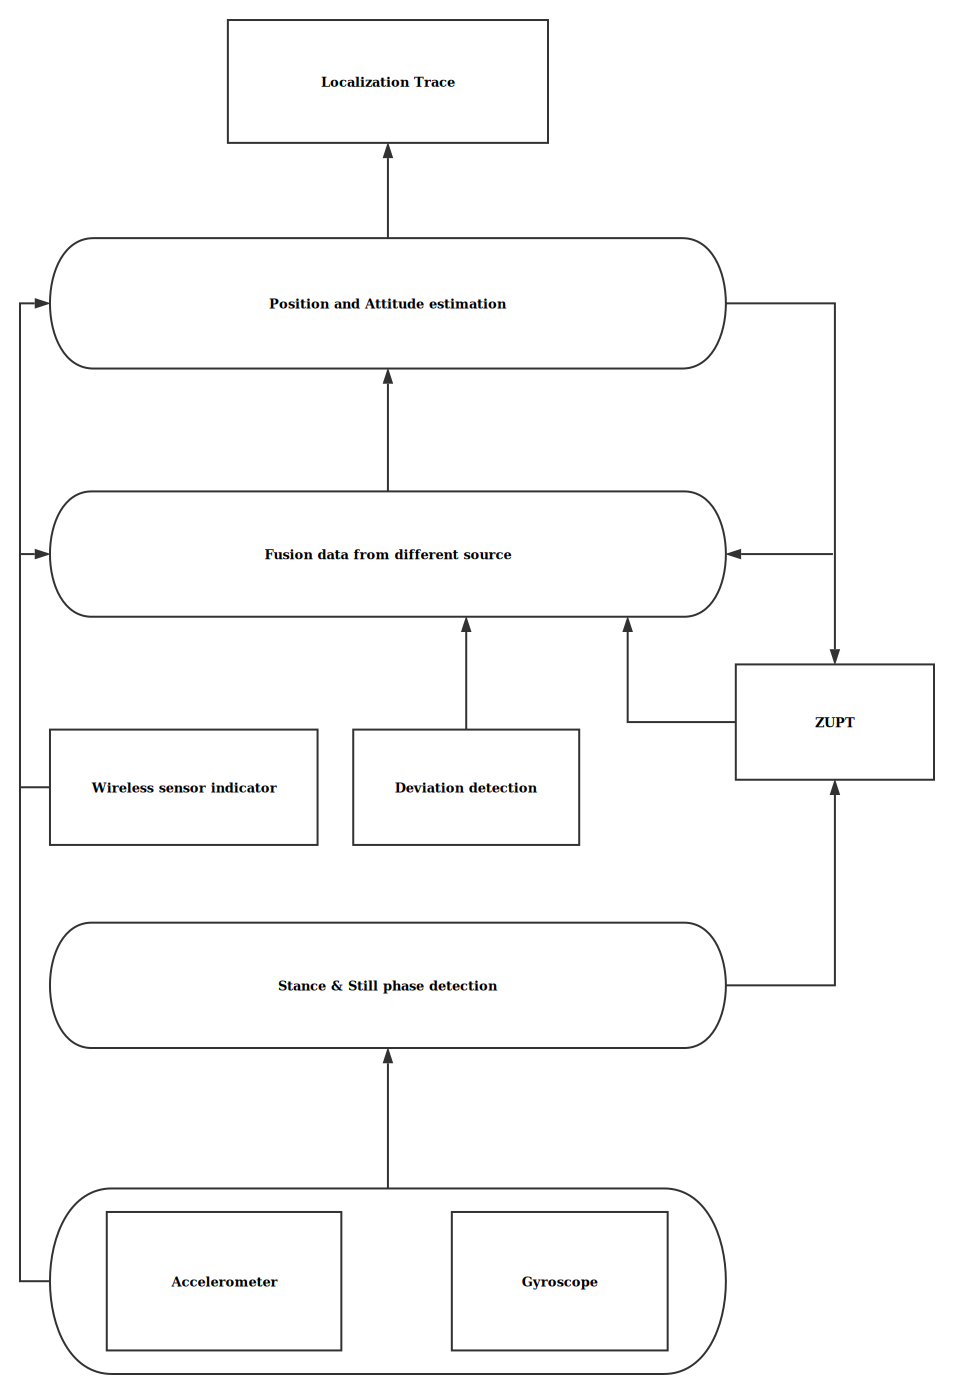
\includegraphics[width=0.8 \linewidth]{pic/systemdiagram.pdf}
      \caption{\bf Application scenario.}
      \label{fig:exitsign}
      \end{figure}

The fire exit sign is part of fire alarming system, which is used to provide evacuation notifications on the evacuation plan \cite{pu2005evacuation}. Kobes et al. examined how people determined evacuation paths during fire-related emergency situations through a series of tests conducted in a hotel building at night \cite{kobes2010way}. They found that 56.3\% of people determined evacuation paths by using exit signs when there was no smoke; however, 81.8\% depended on exit signs for an evacuation path when their visibility was impaired due to smoke. Cho et al. \cite{cho2015automated} proposed an automated direction setting algorithm (ADSA) to trigger dynamic changes in the direction signs so as to reflect real-time fire situations, and to inform evacuees of the directions towards the shortest safe evacuation paths. However, these work remains theoretically and doesn't take the physical path characteristics into consideration. Besides, they assume the evacuee starts from an exit sign, which is not always the case. Solely counting on the light of the direction sign is not sufficient for recognizing a reliable retreat route, as smoke or falling walls may shadow the exit signs and make the route disconnected.


Academic and industry research has taken important steps towards accurate indoor localization using various approaches which can be classified into two classes: infrastructure-based and infrastructure-free. The first class mostly utilize WiFi and lights to localize users. For example, \cite{kumar2014accurate} proposed a WiFi based localization system using Synthetic Aperture Radar (SAR) to emulate large antenna arrays on commodity mobile device. The device can achieve a median error of 39 cm in three dimensional space. \cite{yang2015wearables} presented a solution based on visible light. They use polarization to encode location information of light sources, so that flicking can be avoided. Infrastructure-based solution may achieve nice localization result, however,due to fire, explosion, especially the interruption of power supply and so on, most pre-installed infrastructure would probably not work any more. 

Researchers have also explored infrastructure-free solutions for firefighter localization, such as the Pedestrian dead reckoning (PDR) \cite{nilsson2012foot} \cite{jimenez2009comparison} \cite{beauregard2006pedestrian} . Unfortunately, it is well known that PDR suffers from error accumulation and cannot achieve long term accuracy. Calibrating the result of PDR with some form of landmarks is hence necessary to cope with this problem. For instance, \cite{ruiz2012accurate} describes how to combine PDR with the deployed RFID tags to eliminate the location error. \cite{beauregard2008indoor} developed a particle filter with floor map information included which enhanced the PDR performance. However, such device has limits of range due to self constrain. Moreover, we argue that it is not reasonable to assume that floor plan gives a detailed description for the building, laying emphasis on the details is ill-conceived.

We also note that there have been work on fusing varies technology, like camera, WiFi finger print and sensor tag, as \cite{correa2014enhanced}\cite{gadeke2011pedestrian}\cite{schmid2011fusion}\cite{zheng2014travi}. Zheng \cite{zheng2014travi} provides a vision-guided navigation system integrated with PDR unit and WiFi for trace tracking and motion detection, however it is not capable for buildings on fire. Besides we argue that, WiFi finger print is not always available or stable, which makes it unaccessible for lots of applications. Besides localization, communication is another essential problem involved. The RFID tag based solution is not capable to send localization information out, especially when the firefighters enter the basement where the wireless signals from outside is weakened deeply. 

Actually we can extend exit sign as wireless sensor nodes, which can be used to detect the environment parameters such as smoke density, temperature and poisoned gas, the most important, they can form an wireless sensor network (WSN), and deliver the information collected. Liu \cite{liu2010automatic} et al. proposed a breadcrumb wireless sensor system which can deliver message hop by hop so as to provide a robust communication for the firefighter. Due to the body shadow effect, the signal would be deeply weakened as the body absorbs wireless signal \cite{liu2014providing}. This is a harm point to overcome for reliable delivering message. In this work, we present a novel strategy to use it as heading estimation.

To our best knowledge, most existing WSN based localization work lay much emphasis on devices which are outside from firefighting system, while paying little attention to the device already be used for firefighting, making it not practical or affordable. But in our problem, corresponding network structure with physical distribution calls for extra effort, as on fire environment is volatile. Firefighter may deviate from escape route, detecting the deviation and driving it back is necessary but not easy to fulfill. In addition, signs may not available due to limited quantity, and some signs may be damaged by the fire.  Even worse, as firefighter stands among several signs, how to select an optimal one is also important but  challenging.


\section{SYSTEM DESIGN}

Retreat route selection and navigation for indoor firefighting brings new challenges to system reliability, mainly due to the safety-critical nature and the harsh environment in firefighting applications. To the best of our knowledge, existing solutions like vocal reports are not sufficient to solve this problem. During firefighting, the failure of navigation may result in huge danger that may cost lives of firefighters. Infrastructure-free solutions could not track users with high accuracy for a long period, while landmark based technology is not applicable for this situation, making the system design more challenging. Worse, most pre-installed devices cannot work any more when the main power is down, which is always the case when the building is on fire. How to design a reliable retreat route selection and navigation system under this situation is still unsolved.

In this paper, we propose a novel indoor navigation system for firefighters that consists of: (1) a graph model which builds up main evacuation route map using FESs and update it according to the collected environment information in real time, (2) a motion tracking engine including a PDR unit and a relative ranging unit; (3) an exit sign wireless sensor network that provides communication support and localization landmarks; (4) a fusion algorithm that utilizes the combination of wireless signal and personal movement to better navigation and (5) a novel strategy for heading determination when hopping towards an exit sign on the route.
    %
These components together provide reliable retreat route selection and navigation system in on-fire buildings for firefighters. We describe the system overview and detailed design of each component in the following subsections.

  \subsection{Overview}

    %\subsubsection{A Use Case}
      
    Figure \ref{fig:usecase} demonstrates a use case of SmartFES, where exit signs function as landmarks, combined with intersections of evacuation route segments, we get a full evacuation route map.

    When the firefighter enters the building, he turns on SmartFES and get himself lock-on. As he walks around, the embeded IMU on feet would record the navigation trace, the receiver on body keeps sending periodic broadcast message to estimate the position. If firefighter comes across an exit sign, the absolute position can be determinated as the exit sign's position is known. Besides, signs and wireless connections between can form a graph, which describes the available routes distribution, hence gives an escape route with a sequence of signs for the firefighter. Heading engine tells the heading towards next exit sign by detecting signal strength differences between receivers from the front and the back. Combining with the trace derived from IMU, firefighter is able to know where he is from and where he is going, making it available to reach the next exit sign safely.
      \begin{figure}[!t]
      \centering
      \includegraphics[width=1 \linewidth]{pic/usecaseE.pdf}
      \caption{\bf When a firefighter moves close to an available exit sign, his location is captured and the system quickly find an optimal retreat route as a sequence of signs.}
      \label{fig:usecase}
      \end{figure}

%--------------------------------------------------------------------------------------------------------------
        
    % \subsubsection{Challenge}
      
    The exit sign is not always available on route due to the limited quantity, making it challengable to hop from current position to next exit sign. Considering the complexity of the building on fire, searching a suitable route for escaping is essential to the efficiency and security, yet is not easy. Besides, as the escape route is given as a sequence of signs on the route, but what if the firefighter is not on the route, what should be done to direct him back and how can we tell if the firefighter is really back. Moreover,locating the firefighter on the route is also a big problem, as he may reach a position with several routes intersected, or stand between two signs while lost heading. All these questions together make the navigation for fire fighter challengable to fulfill.

    \subsection{FES Network}
    
    Exit signs are distributed at known position of the building, which can be used as landmarks just as mentioned before. Acoording to the regulation of the firefighting installation standard, evacuation exit sign must contain the storage battery to support the embedded light for at least 90 minutes when the mains is off, which makes it easily to attach a wireless sensor nodes. Hence, we connect the discrete exit sign with wireless signals and get a wireless sensor network.

    The network is organized as reference sensor exit sign, mobile sniffer and base station. The reference sensor exit sign functions as the landmark for evacuation route representation. To address the energy comsuming problem and practical use, we set the reference sensor node in passive mode, which means they only send back localization information when the mobile sniffer requests. The base station is terminal computation center for providing results to incidence commander when making action instruction. The mobile sniffer is carried by firefighter so as to sniffer the wireless signals. All the three kind of devices can forward message packet hence also provide a reliable link for communication.

    Once firefighters arrived at the fire, the commander turns on the base station, joins the wireless sensor network, and collects messages from firefighters with SmartFES mobile sniffers, hence to give them a pre-judge of danger when firefighters enter the on-fire building.

    \subsection{Graph Model}
    {\bf Route Map}    
    Due to volatile decorations such as furnitures, shelves and etc., floor plan can't describe real-time distribution accordingly, making most floor plan based localization system unavailable. We don't put much emphasis on the details of the building, and just focus the evacuation routes map consisted of lines and intersections, which divides the floor into several areas. Once the firefighter received the evacuation command, the system would first search for an exit sign which is easy to reach and effcient for retreating. The retreating process is hence a sequence of exit signs, a natural thought is to reprent the graph with exit signs as vertex, however this would make the problem even more difficult. First we should determinate the existence of edges among signs, second, we need to decide the weight of the edge, which is hard. Last but critical, this would lose some physical information of the route. So we propose a novel model to build a route map with exit signs as landmarks for evacuation route representation.


    As law of firefighting commands, it is the duty of building owners to keep evacuation routes unblocked. Furthermore, the evacuation map should be put on record to the authorities, which makes it available when caught on fire. Figure \ref{fig:usecase} gives an example evacuation map, with gray lines represent route segments and diamonds as exit signs. The empty areas of the map are rooms and open space, where the exact distributions are unknown.

    To model the map mathematically, we treat route segments as edges $E$, intersections of route segments as $V$, and get a represented graph $G(V,E)$. Then we search the efficiency based optimal route from the graph we get. An efficient route is not always the route with shortest distance, as short routes may take much effort to pass through, like requiring many turns. Besides, lacking exit signs would bring much difficulty to walk through the route segment. Taking these factors into consideration, we design the edge weight as following formulas:
    \begin{eqnarray}  
    	f =& d - K m   \\
       w(d,m)=&\left\{   
      \begin{array}{rcl} 
         f  + C,    {f\geq0}\\
         C, {f<0}&
      \end{array}
     \right.  
    \end{eqnarray}
    where $d$ is edge length, $m$ is the number of signs on the edge. As heading estimation at intersections would cost extra effort, hence we add a constant $C$ to represent the effort for determinate the next segment when reached intersection. $K$ is a positive coeffcient to describe the benifit of exit signs. If $K,C=0$, weight of the edge is solely determinated by the length, hence the optimal route searching is turned to be the shortest route searching problem.

    We represent the cost for evacuating from an exit sign $t$ in the middle of edge $(v_i,v_j)$ as following formula:
    \begin{equation}
    \label{eqn:weight}
    cost(t)=min\{cost(v_i) + w_{it}, cost(v_j) + w_{jt}\}\\
    \end{equation}

    where $w_{it}$ and $w_{tj}$ are defined as:
    \begin{equation}
    \left\{
    \begin{array}{rcl}
    w_{it} =&\frac{w(d_{it},m_{it})}{w(d_{it},m_{it}) + w(d_{jt},m_{jt})} w_{ij}\\ \\
    w_{tj} =& \frac{w(d_{jt},m_{jt})} {w(d_{it},m_{it}) + w(d_{jt},m_{jt})}w_{ij}
    \end{array}
    \right.
    \end{equation}

    where $cost(v_i)$ and $cost(v_j)$ are the cost to retreat from instersection $v_i$ and $v_j$, $w_{ij}$ is the weight of the edge $(v_i,v_j)$, $w_{it}$ and $w_{jt}$ are the cost for exit sign $t$ to achieve $v_i$ and $v_j$ correspondly. It's obviously if an exit sign is in coincidence with an intersection, it should have the same cost for retreating.

    Next we present an algorithm for building an evacuation map embedded in the physical route map, and represent the retreat route as a sequence of exit signs.

   {\bf Route search} 
    Dijkstra algorithm is a classical and powerful algorithm for searching shortest path between two vertex, while it can't be applied here directly for following reasons. First, as the building on-fire may have several floors, reprenting and searching a 3-D map is tedious. Second, the quantity of exit signs in the whole building may be large, which would bring much computation for map updating and route searching. Moreover, as there may exist several EXITs, how to select a suitable one from them is also troublesome. 
    \begin{definition}[{\bf Cost based Optimal Evacuation Graph}]      
      For a given graph $G(V,E)$ with $w(d_{ij},m_{ij})$ attached to the edge, where $d_{ij}$ is edge length, $m_{ij}$ is the number of exit signs on edge $(v_i,v_j)$. $ExitStairs=\{ES_1,ES_1,\dots,ES_k\}$,$\vert V \vert = n, \vert E \vert = m$, search a route as a sequence of exit signs on the route towards an exit stair $es \in ExitStairs$ with minimum cost.
    \end{definition}

    \begin{lemma}[Turn 3-D to 2-D path]
    Optimal path searching of a building's 3-D graph G(V,E) is actually a 2-D path searching.
    \end{lemma}

    \begin{proof}[Proof]
      Path search on the ground floor is already a 2-D problem. For the rest floors, path searching can be divided into 3 steps, (1)searching an optimal path towards the stair on that floor, (2)walking through the stair to the ground floor, (3)finding the exit on ground floor. Path searching for each one of the 3 steps is a 2-D problem.
    \end{proof} 
       % build a graph with intersections as vertice, and routes between as edges.
    % consider each exit sign on the route segment. Assign a value to each exit sign accordingly.    
    \begin{algorithm}[!t]
      \label{alg:optRoute}
      \DontPrintSemicolon
      \KwData{Weighted graph $G(V,E,W)$, landmarks $M$, $ExitStairs \subseteq V$.} %
      \KwResult{A cost based evacuation map with exit signs as landmarks}
      \Begin{
     	Merge ExitStairs into one vertex as $start$.\;
     	$T\longleftarrow V\setminus ExitStairs \cup start$\;
     	$adjacent(T,start)\longleftarrow \emptyset$\;
     	\ForEach{vertex $es \in EixtStairs$}{
     		$adjacent(T,start) \longleftarrow adjacent(T,start) \cup adjacent(V,es)$
     	}
        \ForEach{vertex $v \in T $}{
          $cost(start,v) \longleftarrow \infty$ \;
        }    
        $S \longleftarrow \emptyset$\;
        $Q \longleftarrow T$\; 
        $cost(start,start)\longleftarrow 0$\;
        \While{$Q \neq \emptyset$}{
          $u \longleftarrow min\textrm{-}cost\textrm{-}vertex(Q,start)$\;
          $S \longleftarrow S \cup u$\;
          $Q \longleftarrow Q \setminus u$\;
          \For{$v \in adjacent(Q,u) $}{
            $newD \longleftarrow cost(u) + w(u,v)$\;
            \If{$newD < cost(start,v)$}{
              $cost(start,v) \longleftarrow newD$\;
              $parent(start,v) \longleftarrow u$\;
            }
          }
        }   
        $result \leftarrow EvacuateRouteMap(cost,parent,M,G) $\;
        Return $result$\;
      }
      \caption{Cost based optimal route map}
    \end{algorithm}

    Since most evacuation routes contain the stair parts (except ground floor), we can easily transform the problem to a 2-D one, as searching a route towards the stair entrance of the floor, then, feel free to exit through the stair. Besides, the number of EXIT for one floor is limited, hence make make it more easy to search and update the graph in real time. 

    To construct the cost based optimal route map, we use algorithm \ref{alg:optRoute} to build the evacuation route map which doesn't need to search exit stairs one by one, and reduce the complexity of algorithm from $mO(N^2)$ to $O(N^2)$, where $m$ is the number of exit stairs and $N$ is the number of vertice.

     as following step: first, we group all the exit stairs into one node denoted as $start$, and the adjacent vertice of $start$ is the set of the edjacent vertice of the original exit stairs. Then, search the shortest path towards all the rest vertice from the $start$ as Dijkstra algorithm processed. Next, we construct the minimum cost route towards the $start$ for all the intersection vertice. Finally, we use formula \ref{eqn:weight} to calculate the cost for the exit sign in $EvacuateRouteMap(cost,parent,M,G)$. We eventually achieve the cost based optimal evacuation route map embedded in the physical map, each exit sign is attached to a minimun cost for restreating and the route is presented as a sequence of signs just as we promised before.     
 
% the heuristic function + start + goal
    
    The cost based optimal retreat selection is hence as the following steps, first, firefighter would select an accessible exit sign with minimun cost when received the retreating command. After reaching the exit sign, he could follow a sequence of exit signs just as the optimal retreat map provided. Since we have divided the whole route search problem into independend parts, if some exit sign sensed the danger, we denote it as broken one, we remove the edge where the danger is on, and update the map with algorithm \ref{alg:optRoute}. In fact, we need just update the precursor parts of the injured, which would make it even more easier. Besides, if the injured exit sign is on the way to the EXIT, firefighter would follow a new sequence of signs from current position. And if it is not on, firefighter can keep on the old route and we update the map separately.

      % \begin{figure}[!t]
      % \centering
      % \includegraphics[width=1 \linewidth]{pic/dijkstra.pdf}
      % \caption{\bf Group all the exit into one set as Start, then use dijkstra algorithm to calculate the shortest routes towards all the rest vertice}
      % \label{fig:dijkstra}
      % \end{figure}

  \begin{figure}[ht]
  \label{fig:dijkstra}
  \centering
  \includegraphics[width=0.8 \linewidth]{pic/dijkstra.pdf}
  \caption{\bf modified the dijkstra for multi Exit stairs}
  \end{figure}

    \subsection{Motion Engine}
    
    The motion engine utilizes a low-cost inertial measurement uint (IMU) which includes an accelerometer and a gyroscope. We use the accelerometer to calculate the movement and the gyroscope for attitude detection,combined with the geograph charateristic from routes map, hence to give an estimation of the motion for firefighters. Motion engine records the trace between two signs, so as to give a robust tracking for firefighters. However,due to the design and manufacture drawbacks, accelerometer suffers from noise while gyroscope brings drift. Kalman filter havs several disadvantages as discribed in \cite{marins2001extended} \cite{luinge2005measuring}, therefore we utilized an algorithm that has been shown to provide effective performance at low computational expense and at small sampling rates. The algorithm employs quaternion for orientation estimation\cite{madgwick2011estimation}, and it present the orientation result in nearly real-time. The estimated orientation is calculated as following equation:
        % Fuse gyroscope and accelerometer
    % \begin{figure*}[!t]
    %   \centering
    %   \subfigure{\includegraphics[width=0.7 \linewidth]{pic/fusion.pdf}}
    %   \caption{\bf Block diagram representation of the complete orientation filter for an IMU implementation including gyroscope drift compensation}
    %   \label{fig:fusion}
    % \end{figure*}

\begin{figure*}[h]
\centering
\subfigure[{\bf with front side towards the intended sensor exit sign}]{\includegraphics[width=0.4 \linewidth]{pic/bodayshadow.eps}}
\subfigure[{\bf with back side towards the intended sensor exit sign}]{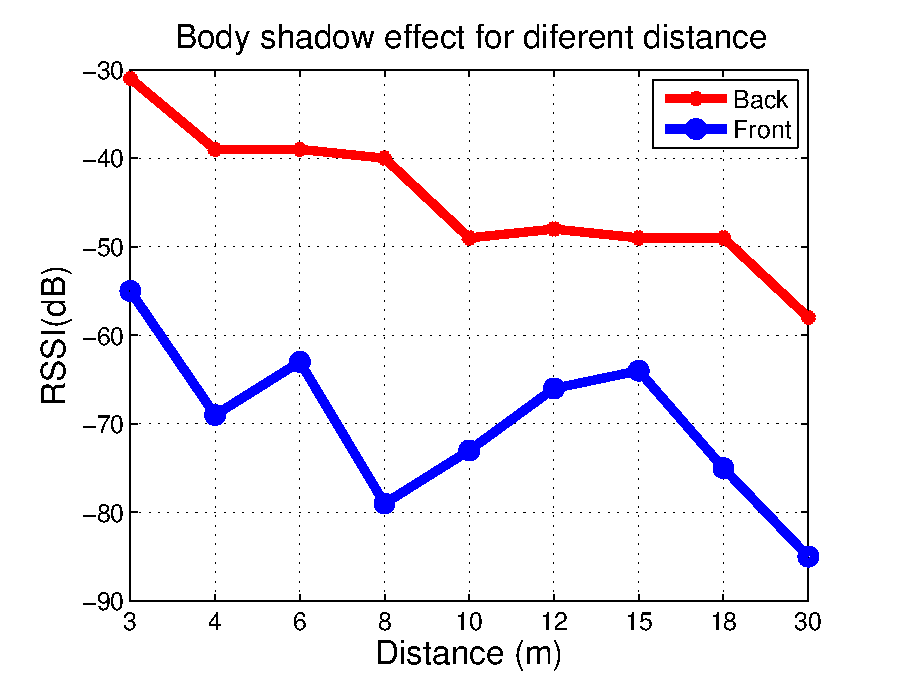
\includegraphics[width=0.4 \linewidth]{pic/boday.eps}}
\label{fig:boday}
\caption{\bf Bodayshadow effect for heading estimation}
\end{figure*}

    \begin{figure}[h]
      \centering
      \includegraphics[width=0.7 \linewidth]{pic/headingEstimation.pdf}
      \caption{\bf Schematic diagram of heading estimation from top view}
    \label{fig:headingEstimation}
    \end{figure}

    \begin{equation}
    \left\{
    \begin{array}{rcl}
     {^{S}_{E}} \hat{q} _{t} &= {^{S}_{E}} \hat{q} _{t-1} + {^{S}_{E}} \dot{q} _{t} \Delta t \\
     {^{S}_{E}} \dot{q} _{t} &= {^{S}_{E}} \dot{q} _{c,t} - \beta \frac{\nabla f}{||\nabla f||}
    \end{array}
    \right. 
    \end{equation}
    where 
    \begin{eqnarray}
    % \begin{array}{rcl} 
    {\nabla f}_g({^{S}_{E}} \hat{q} ,^{S}a) = J^{T}_{g}({^{S}_{E}} {q}){ f}_{g}({^{S}_{E}}\hat{q} ,^{S}a)\\
    ^{S}a_{t} = [ 0 \quad a_{x} \quad a _{y} \quad a _{z} ] \\
    ^{E}g  =  [0 \quad 0\quad 0\quad 1]
    % \end{array}
    \end{eqnarray}

    ${^{S}_{E}} \dot{q} _{c,t}$ is drift error compensated result, which is calculated as following equation:

    \begin{eqnarray}
    % \left\{
    % \begin{array}{rcl}
    ^{S}\omega _{\epsilon,t} =& 2 {^{S}_{E}} \hat{q} {_{est,t-1} ^{*}}\otimes {^{S}_{E}} \hat{q} {_{\epsilon,t}}\\
    ^{S}\omega _{b,t} =& \zeta \sum_{t}{^{S}\omega _{\epsilon,t}\Delta t}\\
    ^{S}\omega _{c,t} =& ^{S}\omega _{t} - ^{S}\omega _{b,t}\\
    {^{S}_{E}} \dot{q} _{c,t} =& \frac{1}{2} {^{S}_{E}} \hat{q} _{est,t-1} \otimes ^{S}\omega _{c,t}
    % \end{array}
    % \right.
    \end{eqnarray}


   In these formulations, ${^{S}_{E}} \hat{q}$ is the orientation of the earth frame relative to the sensor frame, ${^{S}_{E}} \dot{q}$ is the change rate of orientation. Figure \ref{fig:fusion} gives the diagram for the fusion orientation estimation. Even lots of work used the compass to give an global heading estimation within horizontal plan, we argue that it is not applicable in indoor environment, especially the building on fire, as the magnetic field is very sensitive to the spatial structure, and be easily affected by the iron staff, which is very common within the building, like elevator and iron wall. Hence, we give up the compass for use, later we give a strategy for heading estimation towards the intended exit sign which is more reliable.

    %
    By the fusion of accelerometer and gyroscope, we get a sequence of quaternions \{${^{S}_{E}} \hat{q} _{t}\vert t=0,1,2\dots,n$ \}representing orientations in each sample period. We compute accelerations in real world by rotating local sensor frame acceleration to the global earth frame coordinates using following equations:
    %
    \begin{eqnarray}      
      {^E} \hat{a} _{t}= {^{S}_{E}} \hat{q} _{t} \otimes {^S} a _{t} \otimes {^{S}_{E}} \hat{q} {_{t} ^{*}}
    \end{eqnarray}
    %
    In this notation, * denotes conjugate and ${^S} a _{t}$ and ${^E} \hat{a} _{t}$ are the accleration vectors in sensor frame and earth frame, respectively. The velocity in global coordinate is achieved by integrating the transnational acceleration, and we then integrate the velocity to yield position.
    \begin{equation}
      x_t = x_{t-1} + v_{t}\times  \frac{1}{f}
    \end{equation}
    where $x_t$ is position at time $t$, and $x_{t-1}$ is calculated position at time $t-1$, $v_t$ is the velocity at time $t$ and $f$ is the sample rate.

\begin{figure*}[!t]
\centering
\subfigure[Floor plan and distribution of exit signs.] {\includegraphics[width=0.4 \linewidth]{pic/floorPlan.pdf}}
\label{fig:labfloor}
\subfigure[Harware prototype of our implemented system] {\includegraphics[width=0.4 \linewidth]{pic/exitsign.jpg}}
\label{fig:labfloorRep}
\caption{Experimental setup.}
\end{figure*}



      \begin{figure}[!t]
      \centering
      \includegraphics[width=0.8 \linewidth]{pic/floorplanRep.pdf}
      \caption{\bf prototype of our system.}
      \label{fig:usecase}
      \end{figure}

\begin{figure*}
\label{fig:RSSIABCD}
\centering
\begin{minipage}[!t]{1\linewidth}
\centering
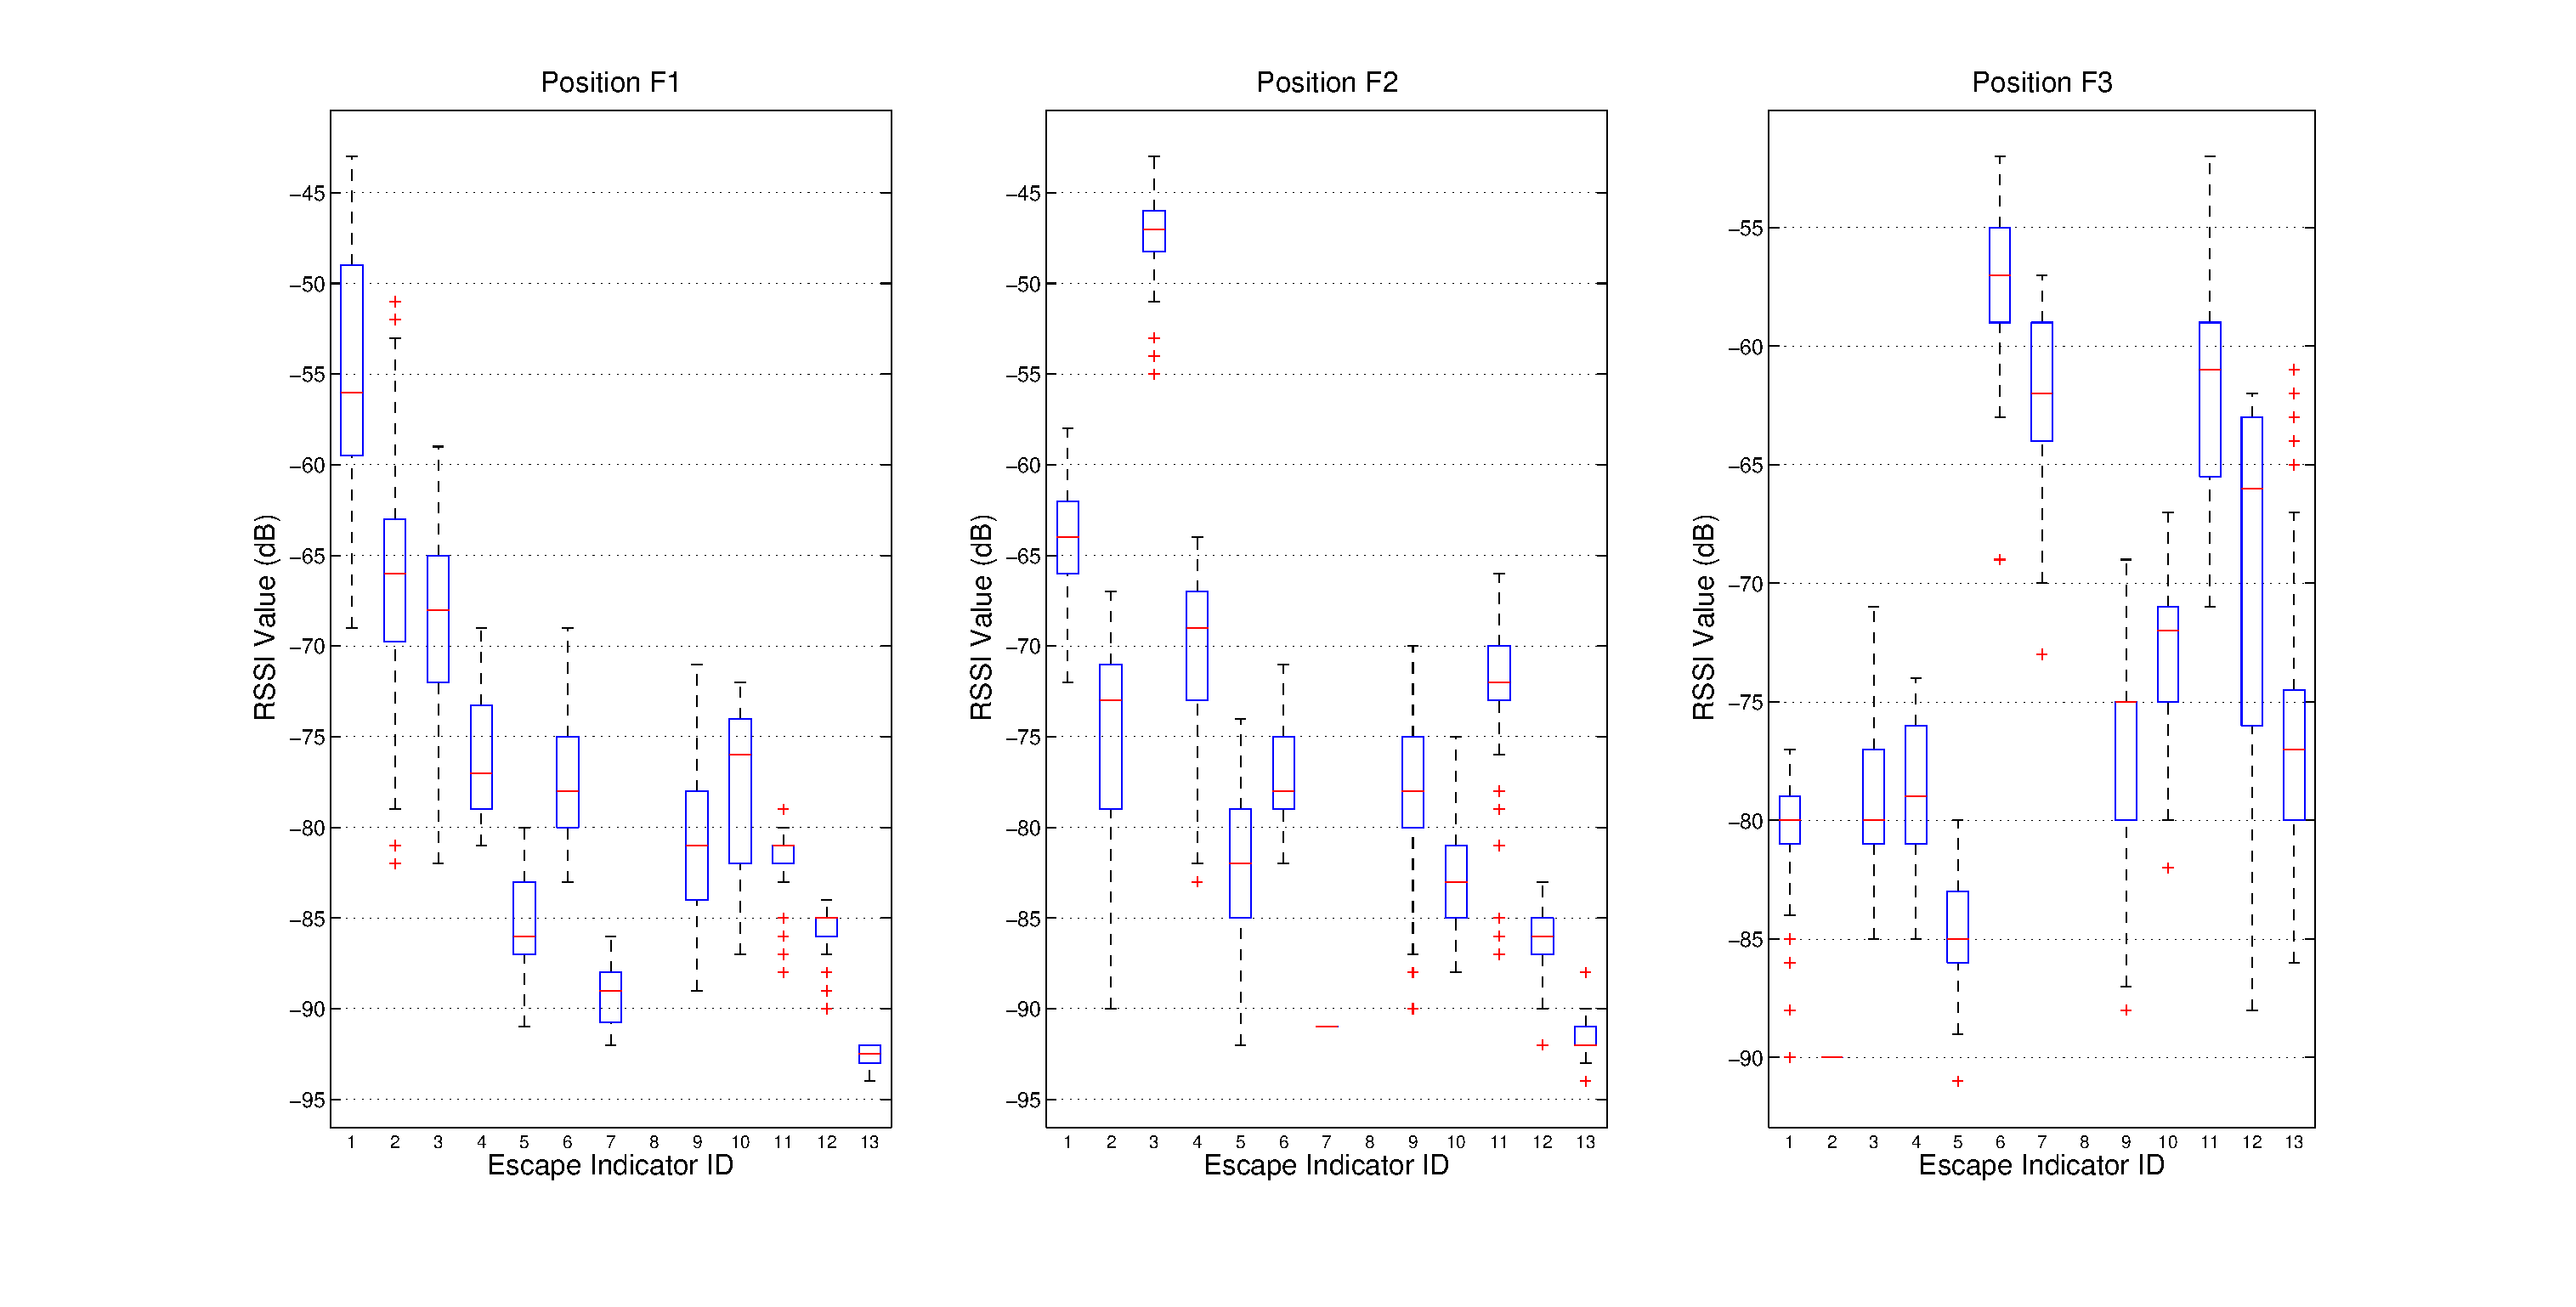
\includegraphics[width=1\linewidth]{pic/RSSIABCD.eps}
\end{minipage}
\caption{Collected RSSI from evaluation points as F1,F2 and F3.}
\end{figure*}


    \subsection{Heading Estimation}
    % Body-shadow effects give an estimation of heading。    
    Received signal strength exit sign (RSSI) is an important parameter in describing the quality of wireless link, which can also be used as the measurement of distance. Lots of researches in indoor application use this technology to fulfill the goal. Previews work mainly focus on the position to locate, while laying little attention on heading, but heading is very essential to the accuracy and robustness of navigation. Knowing whether the intended exit sign is ahead or hehind is very useful for fire fighters to take the first step. To our best knowledge, currently, most available solution count on compass or gyroscope, while neither of them is stable or reliable for indoor application. Others can only conclude heading from the localizaition information, like a trace, but it would bring a time delay for navigation, especially when the initial heading is wrong.


    Considering the body shadow-effect on wireless signal, we present a novel strategy for determinating heading. Figure \ref{fig:headingEstimation} gives a schematic diagram of the strategy, two receivers are set separately at the front and the back of the body, sniffering wireless signals from anchor nodes. Because of the body-shadow effect, two receivers would results in different signal strength, which can easily tell if the anchor nodes is ahead or behind. Note RSSI of front receiver as $frontRSSI$, back as $backRSSI$. As firefighter is on the route, only two direction remains for determinating as front or back. We exame the effect by carrying two receivers in the front and back, the results is present as figure \ref{fig:boday}, it is obviously to see that side which is facing to the anchor node results in greater RSSI value, hence it is easy to distinguish the  direction towards the intended exit sign.

  \section{EVALUATION}

   We have built a prototype of our proposed system to navigate firefighters in harsh indoor environments. The hardware set is shown in figure \ref{fig:exitsign.jpg}, the hardware set includes a mobile sniffer, heading estimator, wireless sensor exit signs, a base station, and a PDR unit. The communication is all based on 2.4GHz chips and the Zigbee protocol. Please refer to \cite{liu2010automatic} for our discussions on using the Zigbee stack and 2.4 GHz based hardware instead of lower frequencies like 900 MHz. The mobile sniffer and heading estimator are wireless sensor nodes with the same hardware design but different embedded software. The PDR unit is covered into a customized 3D-printed box. We only use the accelerometer and gyros, the magnetometers are disabled. The unit is attached to the foot of users. Next we present the performance evaluation details. We first describe the experimental setup, then we examine our system in several apects. Finally, we discuss several observations and explain the evaluation results in detail.
   
\begin{figure*}[h]
\label{fig:rawIMU}
\centering
\subfigure[\bf Trace record by the raw data of IMU] {\includegraphics[width=0.4 \linewidth]{pic/imu.png}}
\subfigure[\bf Trace record by SmartFES] {\includegraphics[width=0.4 \linewidth]{pic/imuINd.png}}
\caption{\bf Benifit of evacuation exit sign for calibration}
\end{figure*}

  \begin{figure}[ht]
  \label{fig:labfloorRepNew}
  \includegraphics[width=1 \linewidth]{pic/floorplanRepNew.pdf}
  \caption{\bf Update the map after exit sign 3 sensed the danger}
  \end{figure}   

  \subsection{setup}
  We conduct the experienment on the 4th floor of the building of Department of Computer Science and Technology at the University of Science and Technology of China. Figure \ref{fig:labfloor} displays the evacuation route map, with gray lines denote the routes and capital letters for intersections of route segments, the exit signs on the route are marked with green diamond. The whole floor is 120m long and 80m wide, with 13 intersections and 3 of them are exit stairs. 

  \subsection{methology}
  We exam our system from several apects as effciency,accuracy and robustness. For effciency, we set the metrix as directly route search from the floor plan. Three firefighters denoted as the F1, F2, and F3 are presented as red pentagrams from diferent positions to retreat from the fire. For the accuracy is examed by recording the walking trace of firefighter F1, which is compared with the inertial navigation system, We also set the exit sign 3 broken so as to simulate detecting the danger, then we test if our system is capable to adapt to the change.

  \subsection{result}
  When the system turns on, exit signs update route segment states according to the collected environment information. The result is then delivered to the base station to present the retreat route map in real time. Algorithm \ref{alg:optRoute} calculates the cost based optimal routes, and assigns each exit sign a direction to next route segment and a value to represent the minimun cost to reach the exit stair. The result is present as Figure \ref{fig:labfloorRep}, which also be used as the user interface for base station.

  For the navigation part, mobile sniffer on firefighter's body keeps sniffering the wireless network to detect the signal strength so as to determinate the accessable exit sign. Figure \ref{fig:RSSIABCD} shows the RSSI value from different sensor exit sign for F1,F2,and F3. For position F1, exit sign 1 gives the maximum RSSI, which means it is nearest one to access. So is for position F2 with the nearest exit sign as 3. Situation for F3 is a little different, for F3 has several accessable exit signs, the system chooses exit sign 7 as next one, because it would bring in minimun cost to reach the exit stair.

  \subsection{discussion}
  Figure \ref{fig:labfloorRep} present the restreat map with a sequence of exit signs. Cost for retreating an exit sign is the sum of each segment's weight. Since the cost may be influenced by 3 factors, distance, number of turns and numeber of exit signs along the route,which can easily conclude the shortest route and the route with minimun turns, are not always the same. It is worthy to do further research to build a better model to exactly discribe the cost.

  The accuracy of our navigation system is parially benifit from the motion fusion algorithm, and it can also remove the cumulation error when came across the exit sign, hence present a even better accuracy for navigation, as figure \ref{fig:rawIMU}. 

  According to the collected sensed danger information, the system can update the retreat map in real time. As the map search problem is effcient as the dijkstra algorithm. As we remove indicator 3 to simulate sensing the danger on the route segment. The system updates the map accordingly, and present the result as \ref{fig:labfloorRepNew}.The result does show our system is robust as it update the retreating map according to the status of route segment changed.




  \section{CONCLUSION}
  This paper presents the design, implementation, and evaluation of an effcient, accurate and robust navigation system, motivated by the important needs on firefighter safety. All previous work failed to provide an effcient, accurate, and reliable solution to navigate firefighters in real time. This paper proposes a novel wireless sensor network system to achieve this goal, by using exit signs as landmarks combined with PDR unit. We described the details of an effcient algorithm for building and updating the retreat map. We fully implemented this system, and apply it in our lab building. We also compared our solution to the sole pedestrian dead reckoning. Evaluation results show that our approach reduces the maximum firefighter location error and provide robust navigation suggestions and significantly outperforms the alternative solution.



% trigger a \newpage just before the given reference
% number - used to balance the columns on the last page
% adjust value as needed - may need to be readjusted if
% the document is modified later
%\IEEEtriggeratref{8}
% The "triggered" command can be changed if desired:
%\IEEEtriggercmd{\enlargethispage{-5in}}

% references section

% can use a bibliography generated by BibTeX as a .bbl file
% BibTeX documentation can be easily obtained at:
% http://mirror.ctan.org/biblio/bibtex/contrib/doc/
% The IEEEtran BibTeX style support page is at:
% http://www.michaelshell.org/tex/ieeetran/bibtex/
%\bibliographystyle{IEEEtran}
% argument is your BibTeX string definitions and bibliography database(s)
%\bibliography{IEEEabrv,../bib/paper}
%
% <OR> manually copy in the resultant .bbl file
% set second argument of \begin to the number of references
% (used to reserve space for the reference number labels box)
  \section{REFERENCE}
    % \begin{thebibliography}{99}
    %   \bibitem{911}
    %   September 11 attacks. \\https://en.wikipedia.org/w/index.php?title=September\_11\_attacks\&oldid=692920730..

    %   \bibitem{TianJinGang}
    %   2015 Tianjin explosions. \\https://en.wikipedia.org/w/index.php?title=2015\_Tianjin\_explosions\&oldid=692552416
      
    %   \bibitem{p25}
    %   Project 25, Sept. 2015.     
    % \end{thebibliography}

    \bibliographystyle{plain}%
      \bibliography{bibfile}


% that's all folks
\end{document}


